\documentclass[11pt, spanish, a4paper, twoside]{article}

% Versión 1.er cuat 2021 Víctor Bettachini < vbettachini@unlam.edu.ar >

\usepackage[T1]{fontenc}
\usepackage[utf8]{inputenc}

\usepackage[spanish, es-tabla]{babel}
% \def\spanishoptions{argentina} % Was macht dass?
% \usepackage{babelbib}
% \selectbiblanguage{spanish}
% \addto\shorthandsspanish{\spanishdeactivate{~<>}}


\usepackage{graphicx}
\graphicspath{{./figuras/}{../LaTeX/}{../figurasLaTeX/}{./figs}}
% \usepackage{float}

\usepackage[arrowdel]{physics}
\newcommand{\pvec}[1]{\vec{#1}\mkern2mu\vphantom{#1}}
% \usepackage{units}
\usepackage[separate-uncertainty= true, multi-part-units= single, range-units= single, range-phrase= {~a~}, locale= FR]{siunitx}
\usepackage{isotope} % $\isotope[A][Z]{X}\to\isotope[A-4][Z-2]{Y}+\isotope[4][2]{\alpha}

\usepackage{tasks}
\usepackage[inline]{enumitem}
% \usepackage{enumerate}

\usepackage{hyperref}

% \usepackage{amsmath}
% \usepackage{amstext}
% \usepackage{amssymb}

\usepackage{tikz}
\usepackage{tikz-3dplot}
\usepackage{tikz-dimline}
\usetikzlibrary{calc}
% \usetikzlibrary{math}
\usetikzlibrary{arrows.meta}
\usetikzlibrary{snakes}
\usetikzlibrary{decorations}
\usetikzlibrary{decorations.pathmorphing}
\usetikzlibrary{patterns}

\usepackage[hmargin=1cm,vmargin=3cm, top= 0.75cm,nohead]{geometry}

\usepackage{lastpage}
\usepackage{fancyhdr}
\pagestyle{fancyplain}
\fancyhf{}
\setlength\headheight{28.7pt} 
\fancyhead[LE, LO]{\textbf{Mecánica Analítica Computacional} }
% \fancyhead[LE, LO]{\textbf{Mecánica General} }
\fancyhead[RE, RO]{\href{https://ingenieria.unlam.edu.ar/}{$\vcenter{\hbox{
\includegraphics[height=1cm]{ambos.pdf}}}$}}
\fancyfoot{\href{https://creativecommons.org/licenses/by-nc-sa/4.0/deed.es_ES}{$\vcenter{\hbox{
\includegraphics[height=0.4cm]{by-nc-sa_80x15.pdf}}}$} \href{https://ingenieria.unlam.edu.ar/}{DIIT - UNLaM}}
\fancyfoot[C]{ {\tiny Actualizado al \today} }
\fancyfoot[RO, LE]{Pág. \thepage/\pageref{LastPage}}
\renewcommand{\headrulewidth}{0pt}
\renewcommand{\footrulewidth}{0pt}

% LTeX: language = es-AR

\begin{document}
\begin{center}
  % \textsc{\large Mecánica general}\\
  \textsc{\large Cuerpo rígido | Distribuciones continuas de masa}
\end{center}

% De poder resolver estos problemas en forma autónoma puede asumir que adquirió los conocimientos mínimos sobre los temas abordados en la semana. No dude en consultar a docentes y compañeros si no puede terminarlos.
% Los problemas marcados con (*) son opcionales.

\begin{enumerate}
	\item 
	\begin{minipage}[t][4.5cm]{0.55\textwidth}
		% \begin{minipage}[t][3.5cm]{0.7\textwidth}
		% Tensor de inercia de un cubo con arista \(b\).
			\textbf{Cubo con arista \(b\)} [Marion (e) ex. 11-3]
			\begin{enumerate}
				\item Calcule el tensor de inercia desde el sistema de ejes \(x_i\) con origen en el centro de masa \(O\).
				\item Use la forma general del teorema de ejes paralelos de Steiner para calcularlo en el sistema \(X_i\) con origen en el vértice \(Q\) 
			\end{enumerate}
		\end{minipage}
		\begin{minipage}[c][1cm][t]{0.4\textwidth}
			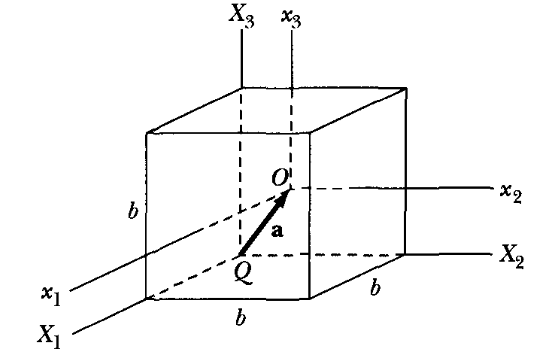
\includegraphics[width=\textwidth]{mFig11-8}
		\end{minipage}


	\item 
		\begin{minipage}[t][4cm]{0.49\textwidth}
			\textbf{Planchuela calada}\\
			En una planchuela de densidad homogénea se calaron dos aberturas en forma simétrica.
			Suspendida desde el punto A \emph{pendulea} en el plano \(x,y\).
			Por eso es relevante conocer su momento de inercia \(I_{zz}\) desde ese punto.
			Cuente con los datos disponibles en un taller: espesor $e$ del material, dimensiones del plano y una $m$ de pesada. 

			Se sugiere seguir esta secuencia:			
		\end{minipage}
		\begin{minipage}[c][2cm][t]{0.45\textwidth}
			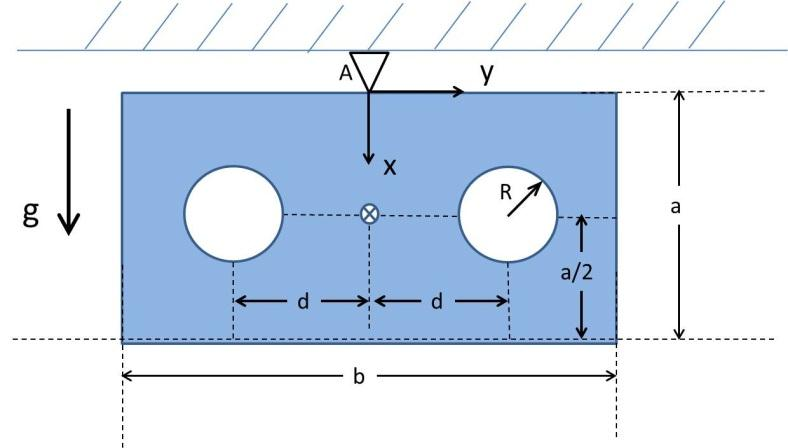
\includegraphics[width=\textwidth]{o-023}
		\end{minipage}
			\begin{enumerate}
				\item Calcular la densidad del metal de la planchuela contemplando el área faltante por los calados.
				\item Idém. \(I_{zz}\) de uno de los calados circulares como si fuera de este metal.
				\item ídem. \(I_{zz}\) de una planchuela sin calado desde su centro de masa.
				\item Trasladar con el teorema de Steiner los \(I_{zz}\) de ambos calados circulares al centro de la planchuela.
				\item Restando al \(I_{zz}\) de la planchuela sin calado el de los círculos obtenga el de la planchuela calada.
				\item Nuevamente con Steiner traslade el \(I_{zz}\) de la planchuela calada al punto de penduleo A.
			\end{enumerate}


			Resultado: 
			\(
			I_{zz} = \frac{m \left(- 12 \pi R^{4} - 6 \pi R^{2} a^{2} - 24 \pi R^{2} d^{2} + 4 a^{3} b + a b^{3}\right)}{12 \left(- 2 \pi R^{2} + a b\right)}
			\) 
			% Respuesta: Se informa el tensor de inercia aunque no requiera calcularle completo.\\
			% \[
			% \overline{\overline{I}} = \left[\begin{matrix}\frac{m \left(6 \pi R^{4} + 24 \pi R^{2} d^{2} - a b^{3}\right)}{12 \cdot \left(2 \pi R^{2} - a b\right)} & 0 & 0\\0 & \frac{m \left(- 3 \pi R^{4} - 3 \pi R^{2} a^{2} + 2 a^{3} b\right)}{6 \left(- 2 \pi R^{2} + a b\right)} & 0\\0 & 0 & \frac{m \left(- 12 \pi R^{4} - 6 \pi R^{2} a^{2} - 24 \pi R^{2} d^{2} + 4 a^{3} b + a b^{3}\right)}{12 \left(- 2 \pi R^{2} + a b\right)}\end{matrix}\right]	
			% \]


	\item 
		\begin{minipage}[t][2.5cm]{0.62\textwidth}
			\textbf{Cilindro rodando en semi-cilindro} [Landau \S 32 6]\\
			%Hallar la energía cinética de un cilindro homogéneo de radio \(a\) que rueda en el interior de una superficie cilíndrica de radio \(R\).
			Hallar la energía cinética de un cilindro homogéneo de radio \(a\) que rueda en el interior de una superficie cilíndrica de radio \(R\).

			Resultado:
			\(
				T = \frac{3 m \left(R - a\right)^{2} \dot{\phi}^{2}}{4}
			\)
		\end{minipage}
		\begin{minipage}[c][1cm][t]{0.3\textwidth}
			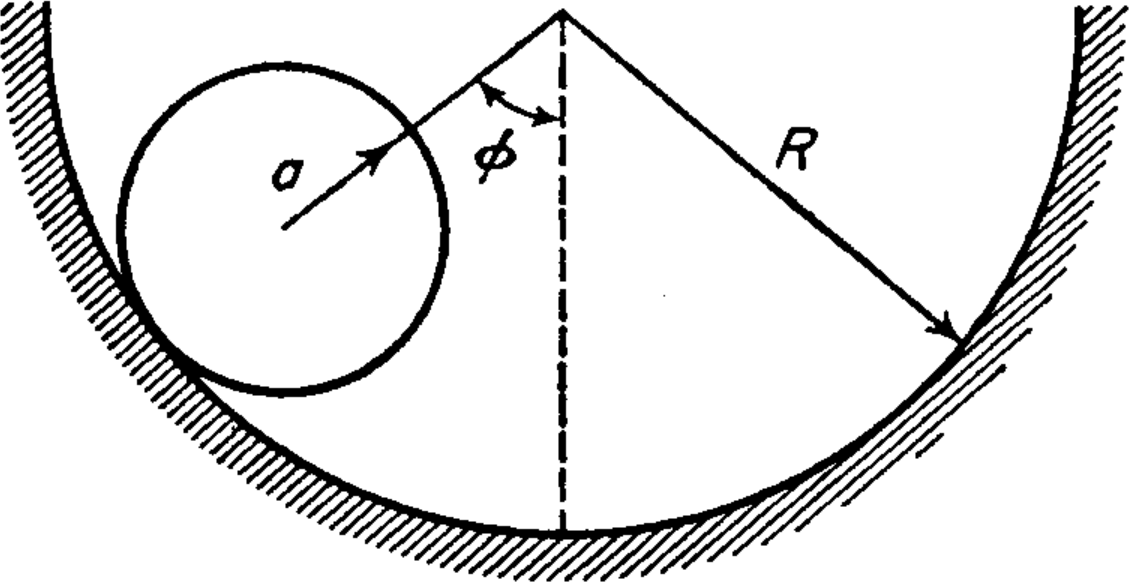
\includegraphics[width=\textwidth]{lFig41}
		\end{minipage}


	\item 
		\begin{minipage}[t][3.5cm]{0.72\textwidth}
			\textbf{Cono circular de altura h y radio de la base R} [Landau \S 32 2e]\begin{enumerate}
				\item Calcule la posición del centro de masa \(O\) desde el vértice \(O'\).
				Recuerde elegir límites de integración en función de la geometría.
				Resultado: \(|\overline{O O'}| = \frac{3}{4} h\).
				\item Calcule los momentos de inercia desde \(O'\).\\
				Resultado: \(I_{x'_3 x'_3} = \frac{3}{10} m R^{2} \qquad I_{x'_1 x'_1} = I_{x'_2 x'_2} = \frac{3 m \left(R^{2} + 4 h^{2}\right)}{20}\)
			\end{enumerate}
			\end{minipage}
			\begin{minipage}[c][1cm][t]{0.2\textwidth}
			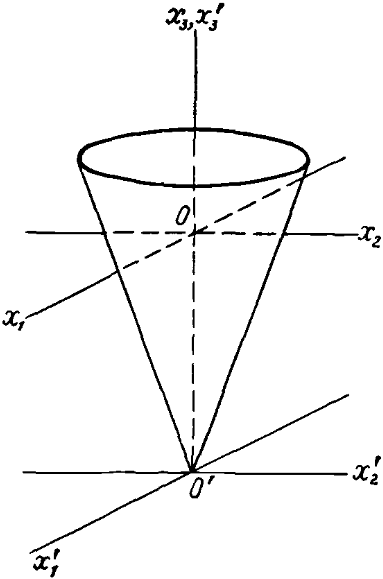
\includegraphics[width=\textwidth]{landauFig38}
		\end{minipage}

	\newpage

	\item 
		\begin{minipage}[t][3.5cm]{0.53\textwidth}
			\textbf{Cono rodante sobre un plano} [Landau \S 32 7]\\
				 El contacto instantáneo con el plano \(X Y\), \(\overline{O A}\), forma los ángulo de \(\theta\) con \(X\) y \(\alpha\) con el eje del cono.
				 El otro dato conocido es la distancia hasta el cento de masa \(a\).
				\begin{enumerate}
					\item Asumiendo conocidos los momentos de inercia desde el vértice en la dirección del eje \(I_3\) y en las perpendiculares \(I_1 = I_2\), calcule la energía cinética.
					Resultado:\\
					\(T = \frac{1}{2} \cos^2(\alpha) I_1 \dot{\theta}^{2} + \frac{1}{2} \frac{\cos^4(\alpha)}{\sin^2(\alpha)} I_3  \dot{\theta}^{2} + \frac{1}{2} \cos^2(\alpha) m a^{2} \dot{\theta}^{2} \)
					\item Exprese en la energía cinética a \(I_{1,2,3}\), \(\alpha\) y \(a\) en función del radio de la base del cono \(R\) y su altura \(h\).
				\end{enumerate}
		\end{minipage}
		\begin{minipage}[c][0cm][t]{0.4\textwidth}
			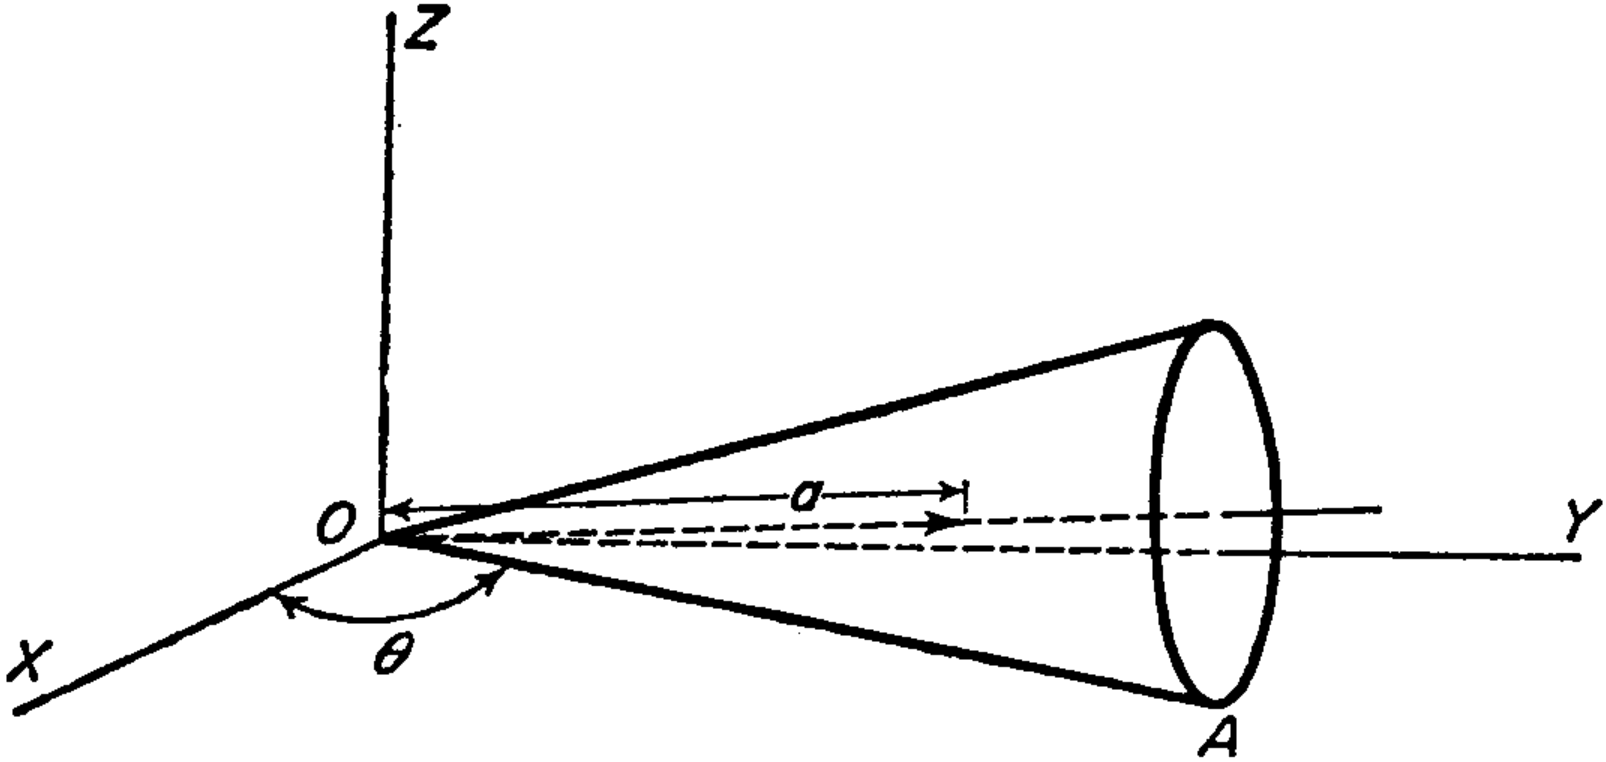
\includegraphics[width=\textwidth]{lFig42}
		\end{minipage}

\end{enumerate}

\end{document}
